\documentclass[../report.tex]{subfiles}

\begin{document}

% Chapter State of the art
% - Concepts (before diving into the protocoles, it is important to understand some concepts)
% - Outlines of the KAPE landscape (all PAKEs, history, overview)
% - Mains PAKEs (differences, improvement, tableau comparatif, pas besoin de décrire les constructions)
%   - EKE
%   - SRP
%   - OPAQUE
%   - KHAPE
% - PAKE choice (and reasons)

% (Attack on PAKEs ?)


% Chapter OPAQUE or Chapter KHAPE (depending on the PAKE choice)
% - detail construction (protocol) of the choosen PAKE

\chapter{State of the art}

\section{History of PAKEs}
\paragraph{EKE and variants (PAK, PPK, PAK-X)}
\paragraph{OKE}
\paragraph{SNAPI}
\paragraph{PEKEP}
\subsection{Symmetric PAKE}
\subsection{Asymmetric PAKE}
\paragraph{SRP}
\paragraph{OPAQUE (2018)}
\paragraph{KHAPE (2021)}





\section{Main PAKEs}

\subsection{\writingFormulationBrut{OPAQUE}}


\paragraph{\writingFormulationBrut{Design}}
Jarecki and al. \cite{OPAQUE_Paper}. introduce the definition of Strong aPake (SaPAKE): an aPake secure against pre-computation attacks.

They provides two modular constructions, called the OPAQUE protocol that allow to builds SaPake protocols. The first construction allow to enhance any aPake to a SaPAKE while the second allow to enhance any Authenticated Key-Exchange (AKE) protocol (that are secure against KCI attacks) to an SaPAKE.
The security of these two construction is based on Oblivious PRF (OPRF) functions \cite{}.

These functions allow for each party, namely the client and the server, to input a secret value and then the client can use the output as a key. Neither party can learn the other party's secret and the server cannot learn the output of the function.

Overall, the OPAQUE protocol allow to secure authentication from the simplest applications to the most sensitive ones.


% \paragraph{\writingNotes{Additional features}}
% 
% In addition to providing a Strong aPAKE protocol, OPRF provides other interesting security features that can be used with OPAQUE.
% 
% 
% "Supports user-side password hardening"
% "has a built-in facility for password-based storage-and-retrieval of secrets and credentials"
% "accommodates a user-transparent server-side threshold implementation"
% "far more secure alternative to the practice of deriving low-entropy secrets directly from a user's password"


\paragraph{\writingFormulationBrut{Construction}}

\begin{figure}[h]
 \centering

 \setlength{\fboxsep}{10pt}
 \setlength{\fboxrule}{1pt}
 \fbox{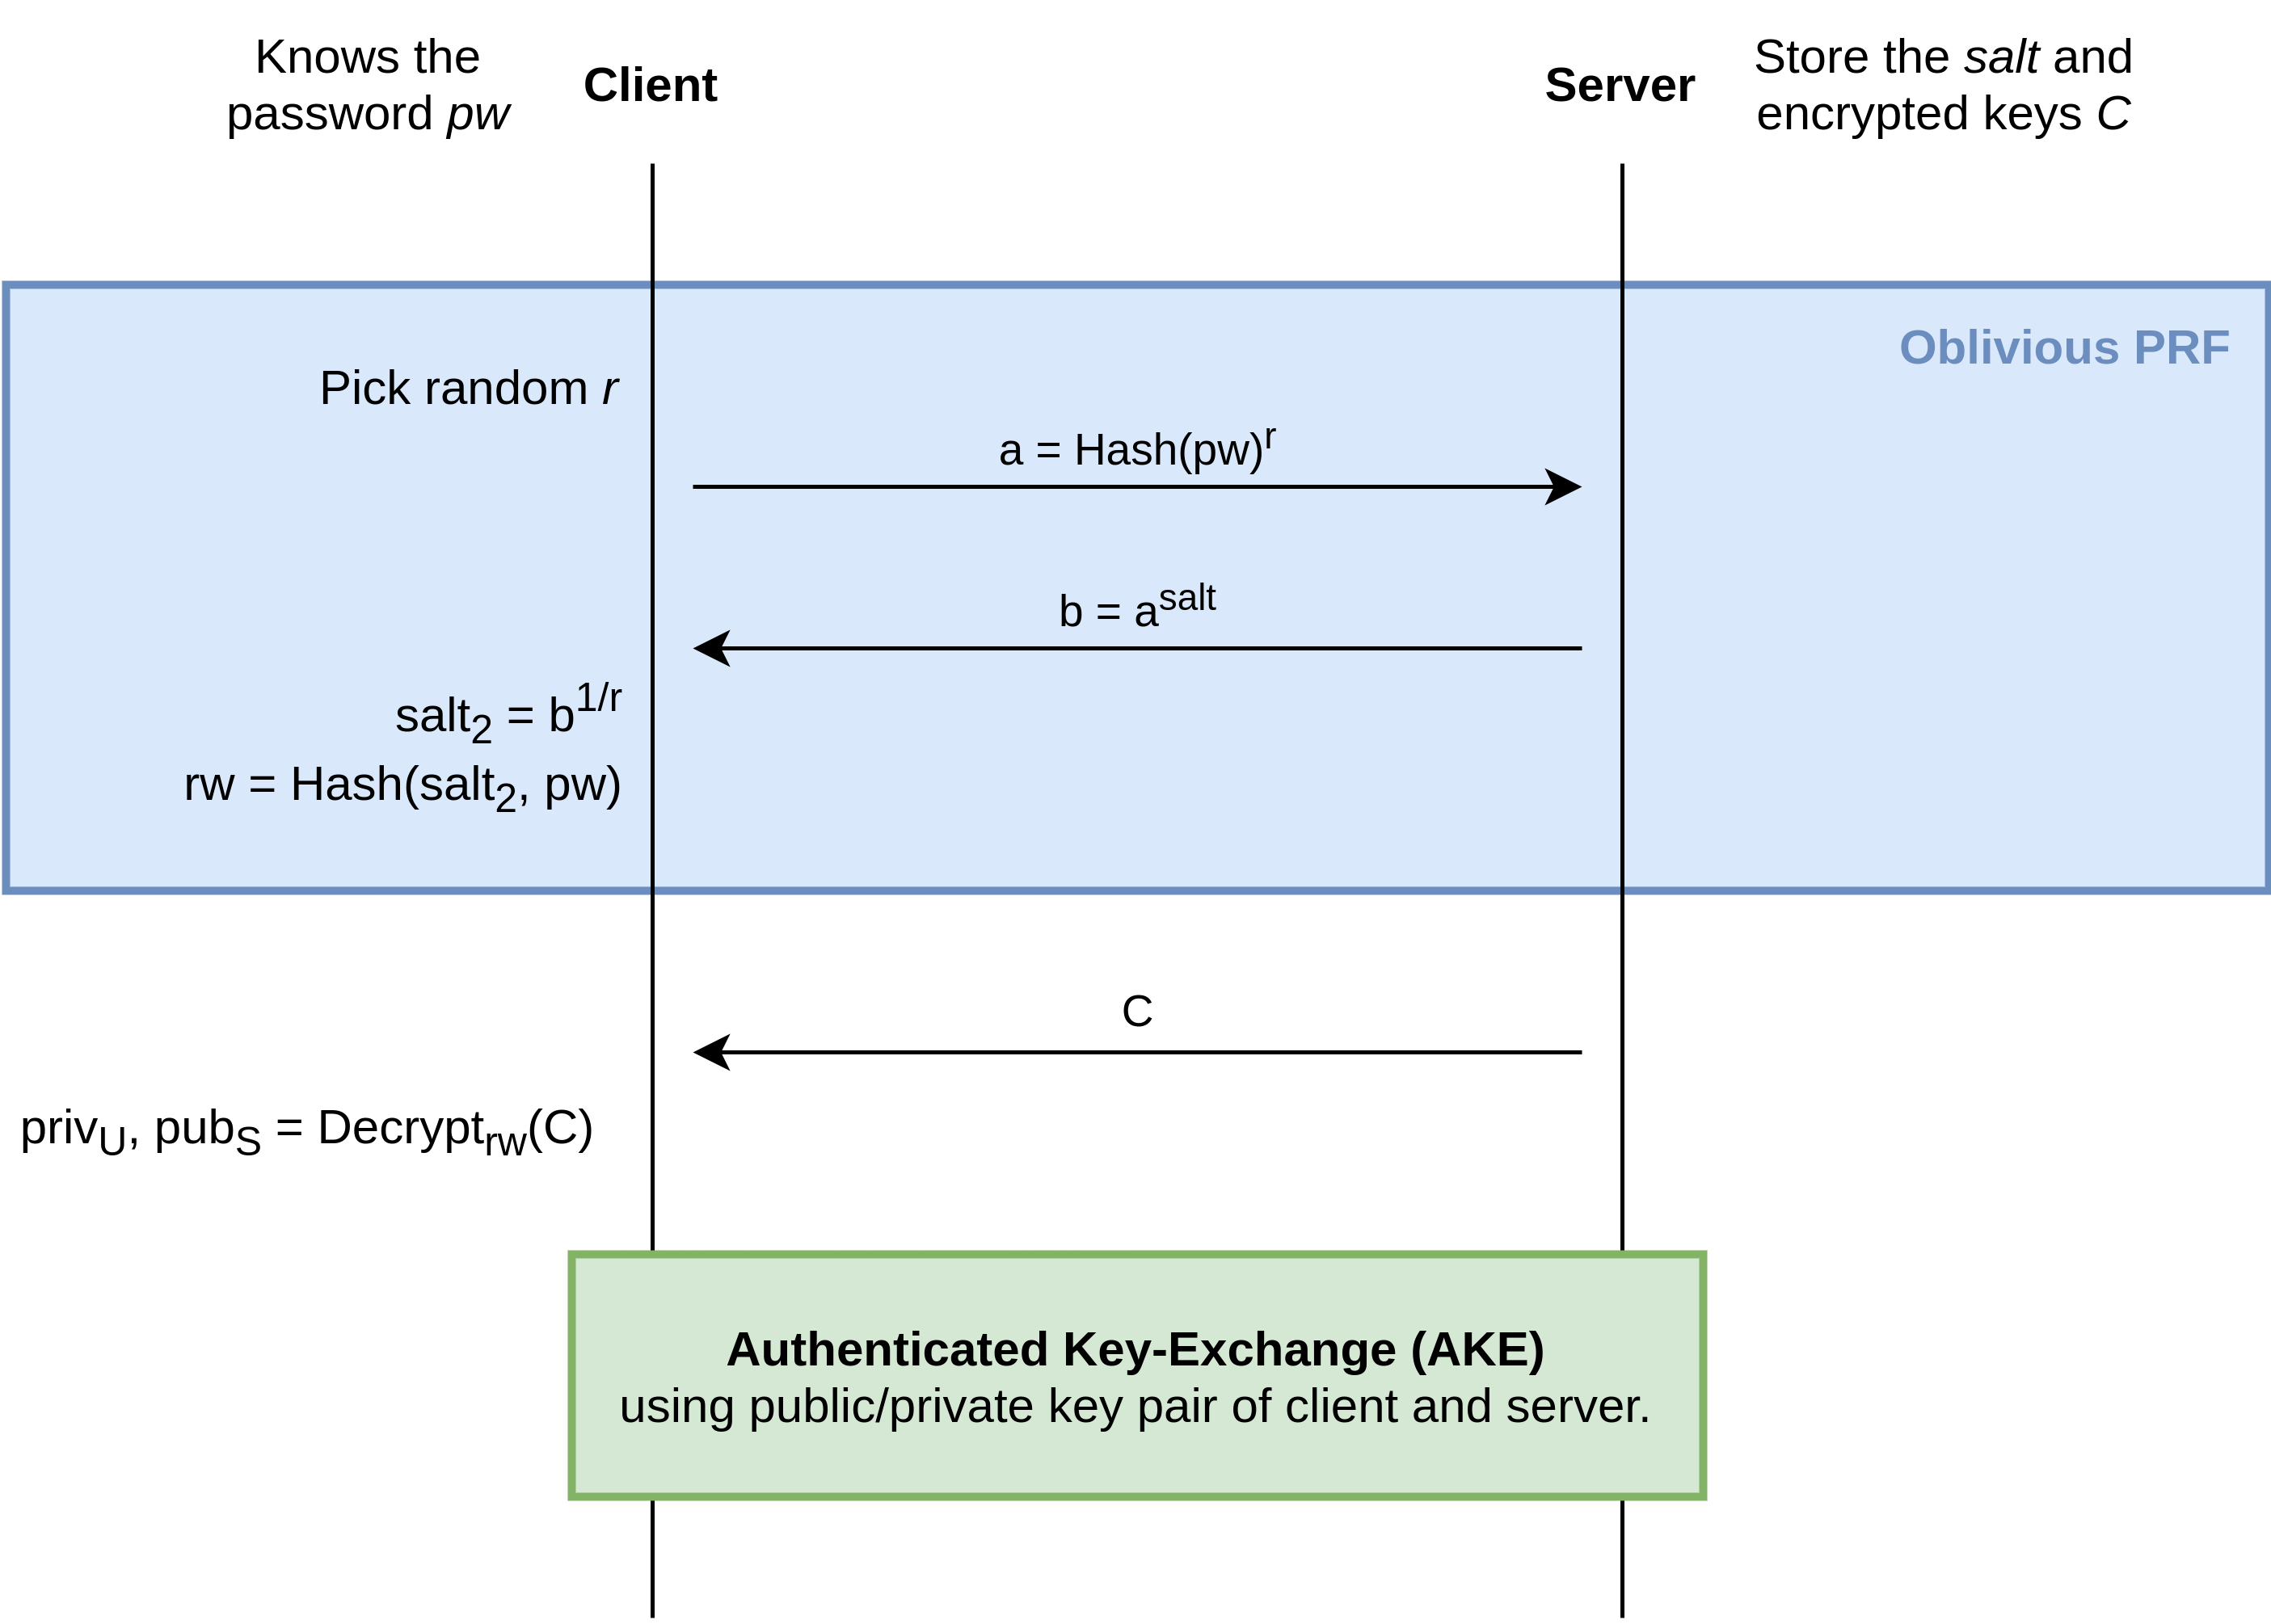
\includegraphics[width=\textwidth-22pt]{OPAQUE.png}}

 \caption{Login process with generic OPAQUE (OPRF-AKE) protocol.}
 \label{fig:OPAQUE_AKE}
\end{figure}

Figure \ref{fig:OPAQUE_AKE} shows the OPAQUE protocol using OPRF and AKE during login process.
The steps are the following :

(1) Generate a random value r to blind the hash of password so that the server cannot retrieve the password from the mapping.
(2) Send result to server.
(3) Server add the salt to the password.
(4) Client calculate the exponant of the inverse of r to unblind the value. He canno't retrieve salt.
(5) With the secret salt salt2, client compute secret key sk.
(6) Server send encrypted keys ek to clients. ek contains server's public key and client's private key encrypted with sk.
(7) If the password entered is correct, client can use sk to decrypt ek and retrieve his private key privU.
(8) With both keys, clients and server can run an authenticated key exchange for mutual authentication.


\paragraph{\writingFormulationBrut{Register}} \label{sec:opaque_register}
The client registration is the only part of the protocol that require a secure channel where both party can authenticated each other.


The protocol is proposed with a server-side registration where the client sends his password through the secure channel. The server generate a salt and compute OPRF function with client's password and salt. Server also generate 2 privates keys (one for the client and one for the server) and their corresponding public key. He encrypt client's private key and server's public key with OPRF output as a key and store the ciphertext.


$C = Encrypt_rw_(client's private key | server's public key)$


This method is not ideal as it require the user to sends it's cleartext password to the server making it vulnerable to miss-handling or server-side vulnerabilities discussed in the introduction.



\cite{OPAQUE_Paper} also note that ideally, one want to implement a client-side registration where the client choose a password and the server choose a secret salt and input them in the OPRF function. The client generate a public/private key pair and the server do the same. Server sends his public key to the client. Client encrypt his private key and server's public key using OPRF output as a key. He then sends the ciphertext to the server with his public key.
This way, the server never see the cleartext password, the OPRF output and the client's private key. This is a major improvement in term of security.

However, this also come with a downside as the server is no longer able to check password rules. This operation needs to be done client-side.


\paragraph{\writingFormulationBrut{Login}}
For the login phase, the client enter it's password in the OPRF and the server send the ciphertext to the client.
If the password entered is correct, the client can decrypt the ciphertext with OPRF output to obtain his private key and the server's public key.
He then use these keys to run a authenticated key exchange with the server (like HMQV ?).

In the other hand, if the password is wrong, the OPRF output is totally different and the ciphertext decryption make the keys uncorrect and the server will refuse it during the key exchange (?). % TODO confirmation



% ====================================================================================



\subsection{\writingFormulationBrut{KHAPE}}
\paragraph{\writingFormulationBrut{Introduction}}

OPAQUE security rely entirely on the strength of the OPRF. If OPRF get broken --- for example by cryptanalysis, quantum attacks or security compromise --- an adversary can compute an offline dictionary attack on the user's password. This is especially critical considering that there is currently no known quantum-safe OPRFs.

KHAPE (for Key-Hiding Asymmetric PakE) \cite{KHAPE_Paper} is a variant to the OPAQUE protocol. Instead of using OPRF as a main tool to archive security, it become an optional part of the protocol and KHAPE use two other concepts to archive security: non-commiting encryption and key-hiding AKE. % TODO non-commiting encryption ??

KHAPE is not a Strong aPAKE like OPAQUE. But it can be made a SaPAKE following the aPAKE to SaPAKE compiler from \cite{OPAQUE_Paper} using OPRF.

So OPRF is optional with KHAPE and just allow to make it a SaPAKE. In addition, it also allow to use OPRF features such as server-side threshold implementation that doesn't require client's change. If OPRF fails, KHAPE just loss these functionalities but the rest of the security remain in contrary to OPAQUE.


% Useful ?
In term of implementation, \cite{KHAPE_Paper} prove that 3DH and HMQV are key-hiding AKE and can be used in KHAPE % TODO see citation in KHAPE_Paper for 3DH and HMQV
It also shows that (some KEM-based AKE like) SKEME can be adapted to archive similar result "if instantiated with a key-hiding KEM". % TODO cites 3DH, HMQV, SKEME papers


% \paragraph{\writingNotes{Mains differences with OPAQUE}}
% - KHAPE is computationally more performant than OPAQUE when the OPRF is not used and the performances become similar when OPRF is used.
% - "KHAPE seems more conducive to post-quantum security via post-quantum key-hiding KEMs."
% 
% - KHAPE allow less AKEs (no signature-based protocols such as SIGMA)
% - KHAPE use ``idea cipher model'', OPAQUE use ``random oracle model'' (stronger ?)
% 
% - with OPAQUE the client learns first if an authentication attempt is succeed or not. with KHAPE, the server learns first which make it easier to count failed attempt in case of an online password guessing attack.
% - KHAPE (without OPRF) cost is ~= same cost as KE cost where OPAQUE cost is about the double of KE cost


% Both client and server needs a public/private key pair to compute a AKE. The client encrypt it's credentials (his private key and server's public key) and store it in the server.



%%% How Key-hiding AKE works ?
%%% Ideal cipher ?



\paragraph{\writingFormulationBrut{Construction}}


\begin{figure}[h]
 \centering
 
 \setlength{\fboxsep}{10pt}
 \setlength{\fboxrule}{1pt}
 \fbox{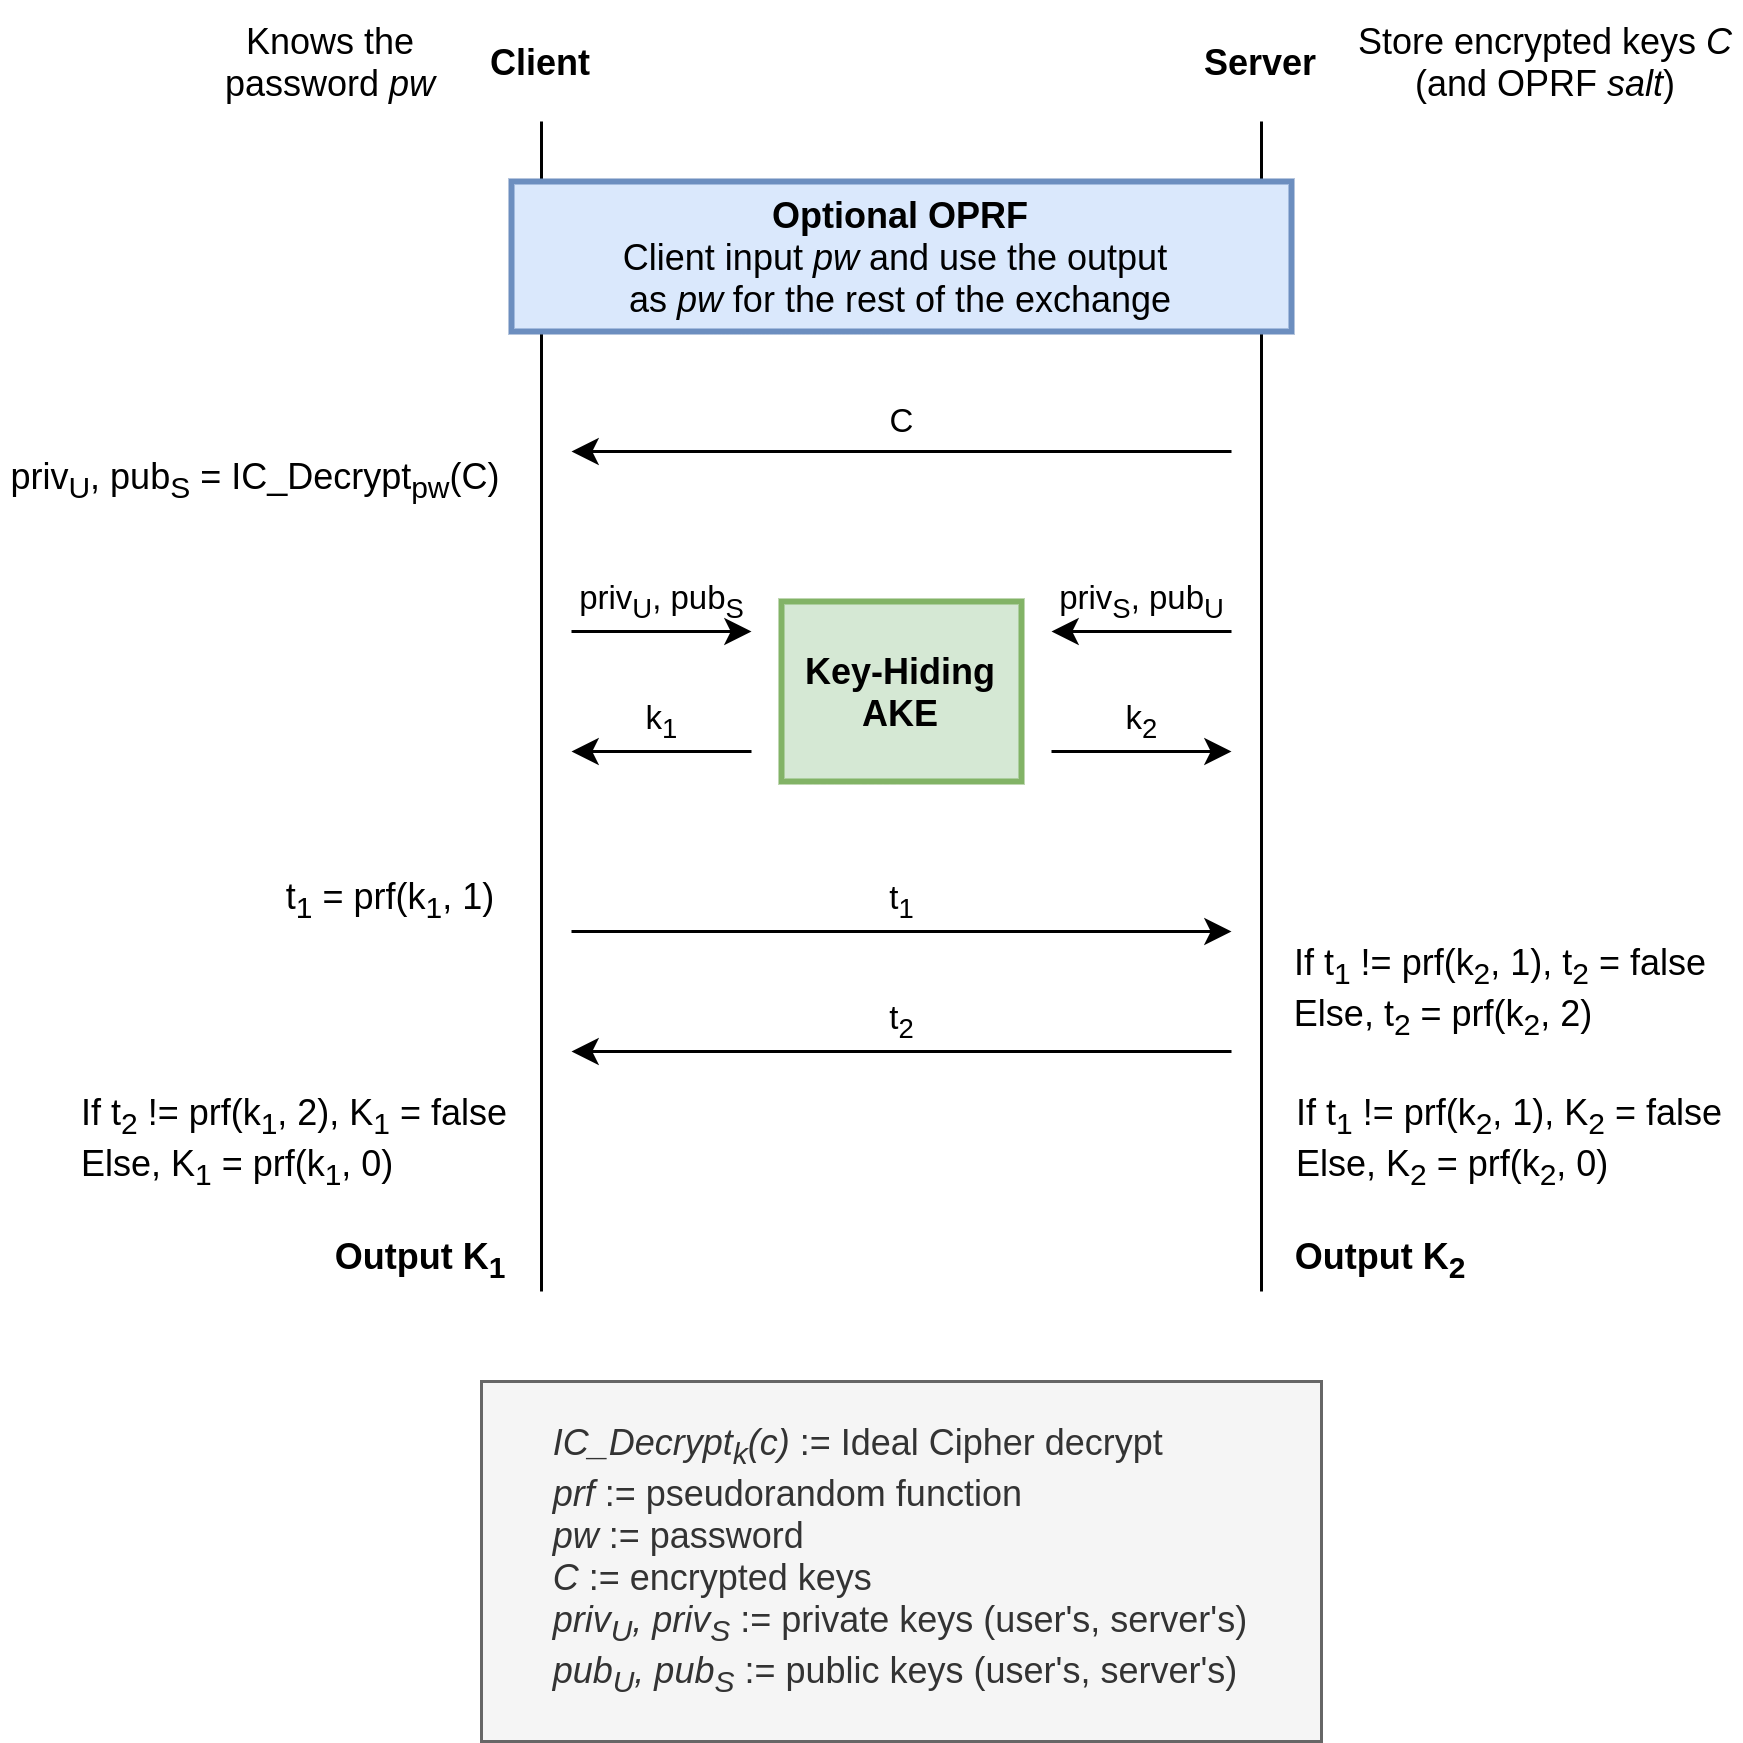
\includegraphics[width=\textwidth-22pt]{KHAPE.png}}
 
 \caption{Login process withn generic KHAPE protocol.}
 \label{fig:Generic_KHAPE}
\end{figure}

Figure \ref{fig:Generic_KHAPE} shows the KHAPE protocol during login process.
The steps are the following :

(1) Optionally, an OPRF can be used to archive Strong aPAKE following the aPAKE to SaPAKE compiler using OPRF from \cite{OPAQUE_Paper}. The OPRF take the client's password and server's salt as an input. Client use the output in place of his password for the rest of the protocol.
(2) Server send the client's encrypted envelop containing the client's private key and server's public key.
(3) Client decrypt the ciphertext using Ideal Cipher encryption schema. He use his password or OPRF output as a key.
(4) Both party use the public/private keys to compute a Key-Hiding Authenticated Key-Exchange.
(5) Mutual key confirmation initiated by the client.

%%% Login and register steps
\paragraph{\writingFormulationBrut{Login}}

When the client want to login, the server sends its encrypted credentials and the client use it's password to decrypt the credentials (with or without OPRF depending on the implementation). Then he can us his credentials to compute a Key-Hiding AKE with the server.

Both party finish with a mutual key confirmation initiated by the client.


\paragraph{\writingFormulationBrut{Register}}
KHAPE has the same problem that is addressed in \ref{sec:opaque_register}.
The protocol propose a server-side register which is less than ideal because the server can see client's password and client's private key in cleartext at register.

Instead, the paper propose a client-side registration process.



% ====================================================================================



\section{\writingNotes{Comparing mains solutions}}

This section compare the mains PAKEs on their security guarantees and performances. Details and comments on each criteria can be found on Section \ref{sec:comparison_details}.

\begin{center}
   \begin{tabular}{ | c | p{8cm} || p{1cm} | p{1cm} | p{2cm} | p{2cm} | }
     \hline
     \textbf{\#} & \textbf{Criteria} & \textbf{EKE} & \textbf{SRP} & \textbf{OPAQUE} & \textbf{KHAPE} \\ \hline
     
     % Content :
     
     % Qualities (security guarantees)
     
     10 & Server doesn't store password in cleartext & x & x & Yes & Yes \\ \hline
     1 & Avoid sending cleartext password to the server & x & x & Yes (May be required during register depending on the implementation) & Yes (May be required during register depending on the implementation) \\ \hline
     2 & Secure against pre-computation attacks & x & x & Yes & Yes, if using OPRF \\ \hline
     3 & Server doesn't send salt in cleartext & x & x & Yes & Yes (OPRF) (without OPRF there is no salt) \\ \hline
     4 & Forward secrecy & x & x & Yes, Full FS & Yes, Full FS \\ \hline
     5 & Mutual authentication & x & x & Yes & Yes \\ \hline
     6 & PKI-free & x & x & Yes, except during register & Yes, except during register \\ \hline
     7 & User-side password hardening & x & x & Yes & Yes, if using OPRF \\ \hline
     8 & Built-in mechanism to store client's secrets on the server & x & x & Yes & Yes \\ \hline
     9 & Server threshold implementation & x & x & Yes, user-transparent & Yes, if using OPRF \\ \hline
     11 & Resistant upon Oblivious PRF compromise & x & x & No, entire security is compromised & Fall back to non-strong aPAKE \\ \hline
     12 & Standardization status & x & x & Internet standard draft \cite{OPAQUE_Standard_Draft} & Crypto 2021 Paper \cite{KHAPE_Paper} \\ \hline
     13 & Security proof & x & x & Yes, in a very strong model (random oracle model ?) & Yes (idea cipher model) \\ \hline
     
     \end{tabular}
 \end{center}
 
\begin{center}
   \begin{tabular}{ | c | p{8cm} || p{1cm} | p{1cm} | p{2cm} | p{2cm} | }
     \hline
     \textbf{\#} & \textbf{Criteria} & \textbf{EKE} & \textbf{SRP} & \textbf{OPAQUE} & \textbf{KHAPE} \\ \hline
     % Performances
     
     14 & Easily adaptable to elliptic curves & x & x & Yes & Yes ? \\ \hline
     15 & Number of messages & x & x & 3 & 4 (3 if client initiate) \\ \hline
     16 & Number of exponentiations & x & x & 3 or 4 ? & 2 + 1 hash-to-curve \\ \hline
     20 & Computational cost compared to a KE (see \cite{KHAPE_Paper} presentation) & 1x & x & 2x & 1x without OPRF, 2x with OPRF \\ \hline
     17 & Patented & Yes, expired in 2011 ? & x & No & No \\ \hline
     18 & Year published & x & x & 2018 & 2021 \\ \hline
     19 & Got broken & x & x & x & x \\ \hline

     \end{tabular}
 \end{center}
 
\subsection{Details} \label{sec:comparison_details}



\paragraph{\writingFormulationClean{10. Server doesn't store password in cleartext.}}
This is the main security property of asymmetric PAKE \cite{aPAKE_Formalized}. Server doesn't have to store password in cleartext which should make it more resilient in case of server compromise. Adversary has to compute an offline attack to retrieve passwords from the compromised server.

\paragraph{\writingFormulationBrut{1. Avoid sending password in cleartext to the server.}}
Even though it seems similar to criteria 1, it's not. Criteria 1 is about password storage but this criteria is about password transmission. Transmissions and storage of the password are vulnerable to different attacks vectors.
The server don't receive password in cleartext which avoid any miss-handling vulnerabilities such as logging or caching cleartext password on the server.

\paragraph{\writingFormulationClean{2. Secure against pre-computation attacks.}}
This is the main security property of Strong aPAKE \cite{OPAQUE_Paper}. The server doesn't leak any data (generally the salt) that could allow an attacker to perform a pre-computation attack. This attack allow an attacker to compute a table \emph{before} the server even get compromised. Once the attacker succeed in compromising the server, he can use the pre-computed table to retrieve the passwords \emph{instantaneously}. So this protection force the attacker to perform an offline dictionary attack after successful server compromise. % This vulnerability weaken the initial benefit of using an aPAKE \cite{aPAKE_Formalized} and even make password-over-TLS more secure \cite{OPAQUE_Paper} (than aPAKE vulnerable to pre-computation attacks).

\paragraph{\writingNotes{3. Server doesn't send salt in cleartext.}}
Same as 2.

\paragraph{\writingFormulationClean{4. Forward secrecy.}}
In key-exchange protocol, Forward Secrecy (also called Full Forward Secrecy or Perfect Forward Secrecy) ensure that upon compromise of any long term key used to negotiate sessions key, an attacker cannot compromise previous session keys.
In details key-exchange protocol use long-lived keys to authenticate the user and short-lived keys to encrypt sessions. With Forward Secrecy, an attacker that successfully compromised a long-lived key cannot retrieve any previous session data even if he recorded the previous encrypted transmissions. % TODO cite Duc CAA 05-password ?

\paragraph{\writingFormulationClean{5. Mutual authentication.}}
Mutual authentication explicit that user must be authenticated to the server but also that the server must authenticate itself to the user to avoid that an adversary impersonate the server to maliciously communicate with the client.

\paragraph{\writingFormulationBrut{6. PKI-free.}}
The transmissions between client and server doesn't require to be secured with PKI. This is a big improvement over classical authentication method (Password-over-TLS) considering the occurrence of PKI failures nowadays. % "PKI failures include stealing of server private keys, software that does not verify certificates correctly, users that accept invalid or suspicious certificates, certificates issued by rogue CAs, servers that share their TLS keys with others e.g., CDN providers or security monitoring software, information (including passwords) that traverses networks in plaintext form after TLS termination; and more."

\paragraph{\writingFormulationClean{7. User-side password hardening.}}
User can use password hardening technique to increase the cost of an offline attacks if the server get compromised. This is done by using ressource-heavy functions such as Scrypt \cite{Scrypt_Paper} or Argon2 \cite{Argon2_Paper} instead of computing a simple and efficient hash. These functions allows to drastically slows down hashing process and so making offline attacks and online guessing attack much slower.

\paragraph{\writingNotes{8. Built-in mechanism to store client's secrets on the server.}}
OPAQUE "has a built-in facility for password-based storage-and-retrieval of secrets and credentials"
~~New protocol such as OPAQUE and KHAPE use client-side decryption of server-stored ciphertext to retrieve key. This allow to run exchange in an unsecure channel because...

\paragraph{\writingNotes{9. Server threshold implementation.}}
OPAQUE "accommodates a user-transparent server-side threshold implementation"

\paragraph{\writingFormulationClean{11. Resistant upon Oblivious PRF compromise.}}
If OPRF breaks for exemple by cryptanalysis, security compromise or even quantum attacks, the consequences could be disastrous depending on the way it is used. This is especially important because there is ``currently no known efficient OPRFs considered to be quantum safe'' \cite{KHAPE_Paper}.
OPAQUE use OPRF as a main tool to builds Strong aPAKE. If OPRF breaks, the client's password is vulnerable to a offline dictionary attack.
KHAPE has a weaker reliance on OPRF. It is optional and only used to archive Strong aPAKE. If OPRF breaks, KHAPE only fall back to a non-strong aPAKE (making it vulnerable to pre-computation attacks). 
This make KHAPE more resistant to OPRF compromise than OPAQUE. 

\paragraph{12. Standardization status.}

\paragraph{\writingNotes{13. Security proof.}}
OPAQUE "security proof in a very strong model"

\paragraph{14. Easily adaptable to elliptic curves.}


\paragraph{15. Number of messages.}


\paragraph{16. Number of exponentiations.}


\paragraph{17. Patented.}


\paragraph{18. Release date.}


\paragraph{19. Version.}


\paragraph{20. Got broken.}



\end{document}
